\documentclass[a4paper, 12pt]{article}
\usepackage{listings}
\usepackage{pdfpages}
\begin{document}
\lstset{ numbers=left, basicstyle=\footnotesize, breaklines, tabsize=2, literate={\ \ }{{\ }}1}
Abstract

In dieser Arbeit werden verschiedene Methoden für die Farberkennung eines Rubiks Cubes verglichen. Dabei werden unter anderem verschiedene Farbräume und Methoden für die Zuordnung eines Feldes zu einer Mitte angeschaut. 
\tableofcontents
\newpage
\section{Einleitung}
In dieser Arbeit wurde versucht, eine Software zu programmieren, die einen Rubiks Cube möglichst gut erkennen soll. Dabei werden Probleme untersucht, die im Gebiet der Farberkennung auftreten können. Dabei werden verschiedene Lösungsansätze miteinander verglichen und es wird erklärt, wie sie im Code angewandt wurden.
\subsection{Rubiks Cube}
Um die Farben eines Rubiks Cubes zu erkennen, muss erst einmal klar sein, wie er überhaupt aufgebaut ist. Ein Rubiks Cube (im Folgenden Würfel genannt) besteht aus 26 Steinen. Diese sind in einer 3x3x3-Würfelform angeordnet, in der der Mittlere Würfel fehlt. Die Steine sind so mit sechs verschiedenen Farben gefärbt, dass jede Seite des Würfels eine Farbe hat (vgl. Abbildung). Dabei existieren insgesamt sechs Mittelsteine, auf jeder Seite einer, die je eine einzige gefärbte Fläche (im Folgenden Mitte genannt) haben. Diese Mitten haben jeweils eine der sechs Farben. Sie ändern beim Verdrehen des Würfels ihre relative Position zueinander nicht. Neben den Mittelsteinen gibt es auch noch Seitensteine. Diese haben jeweils zwei oder drei gefärbte Flächen. So eine Fläche wird im Folgenden "Seite" genannt. 
\subsection{grundliegende Idee}
Die grundliegende Idee ist die, dass der Rubiks Cube immer an einem Fixen Punkt festgemacht wird, und dann von zwei gegenüberliegenden Kameras fotografiert wird. So sind die Felder des Würfels immer an der gleichen Stelle im Bild, und es braucht keine Mustererkennung, um die Felder zu finden. U/m die Felder dann einer Farbe zuzuordnen, werden keine im vorderein definierten Farben verwendet, sondern es werden die Farbwerte der Mittelsteine herausgelesen, und die restlichen Felder werden dann diesen zugeordnet. So wird vermieden, dass man bei jedem neuen Würfel, der andere Farben besitzt, wieder mühselig die richtigen Farbwerte suchen muss, um die Definitionsbereiche zu erstellen. Wenn ausserdem die Lichtverhältnisse  mal etwas dunkler oder heller sind, wird dies dann automatisch miteinberechnet, da die Mitten dann auch dunkler sind. 
\section{Code}
\subsection{Farbräume}
Zuallererst musste festgelegt werden, wie die Farben der Steine aus dem Bild ausgelesen werden. Dafür muss man zuerst verstehen, wie Farben auf einem Bild überhaupt dargestellt werden. Dies geschieht auf einem Computer mithilfe eines Farbraumes. Ein Farbraum ist eine fest definierte Anzahl an Farben, die oft mithilfe von drei Variablen beschrieben werden. Eine Bilddatei enthält somit nur Farben, die durch eine Kombination der drei Variablen erstellt werden kann.(QUELLENANGABE FARBRAUM) Diese Variablenwerte können dann ohne Probleme ausgelesen und miteinander verglichen werden. Zwei der gängigsten Farbräume, die hier miteinander verglichen werden, sind der RGB- und der HSV-Farbraum. 
\subsubsection{RGB}
RGB ist der Standard-Farbraum, für die digitale Bildwiedergabe. Er setzt sich aus drei Werten für Rot, Grün, und Blau zusammen. Die Werte gehen jeweils von 0 bis 255, wobei die Farbe bei 0 nicht vorhanden ist, und bei 255 die Farbe mit voller Intensität leuchtet. (0, 0, 0) ist somit schwarz und (255, 255, 255) ist weiss. Der gesamte Farbraum lässt sich als Würfel in einem Koordinatensystem darstellen, wobei die Achsen jeweils die Intensität einer Farbe beschreiben.

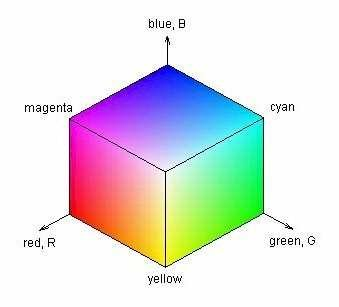
\includegraphics[scale=0.5]{RGB_Wuerfel}

 Der RGB-Farbraum ist ein additiver Farbraum, was bedeutet, dass bei nichts angefangen wird, und je höher die Werte werden, desto mehr Farbe vorhanden ist. Deshalb wird RGB auch bei vielen Arten von Beleuchtung verwendet, wie Fernseher und Computerbildschirme, die ihre Pixel mit roten, grünen und blauen LEDs beleuchten. Auch der Mensch erkennt Farben auf diese Weise, da im Auge Rezeptoren vorhanden sind, die empfindlich auf die Wellenlängen von Rot, Grün und Blau sind.
\subsubsection{HSV}
Der HSV-Farbraum setzt sich aus den Werten "Hue", "Saturation" und "Value" zusammen. Hue ist ein Wert für den Farbton, und geht standardmässig von 0 bis 179. Ausserdem ist der Wertebereich von Hue kreisförmig, was heisst, dass 0 und 179 nebeneinander sind und es somit kein Anfang oder Ende gibt. "Saturation" beschreibt die Sättigung und Intensität der Farbe und geht von 0 bis 255, wobei 0 keine Sättigung und somit Weiss bedeutet und bei 255 die Farbe vollends vorhanden ist. "Value" ist ein Mass für die Helligkeit und reicht ebenfalls von 0 bis 255. Wenn der Value bei null ist, dann spielt es keine Rolle was der Farbton ist, und die Farbe wird schwarz. Je höher der Value dann geht, desto heller wird die Farbe. Der HSV-Farbraum wird häufig in Form eines Zylinders visualisiert.

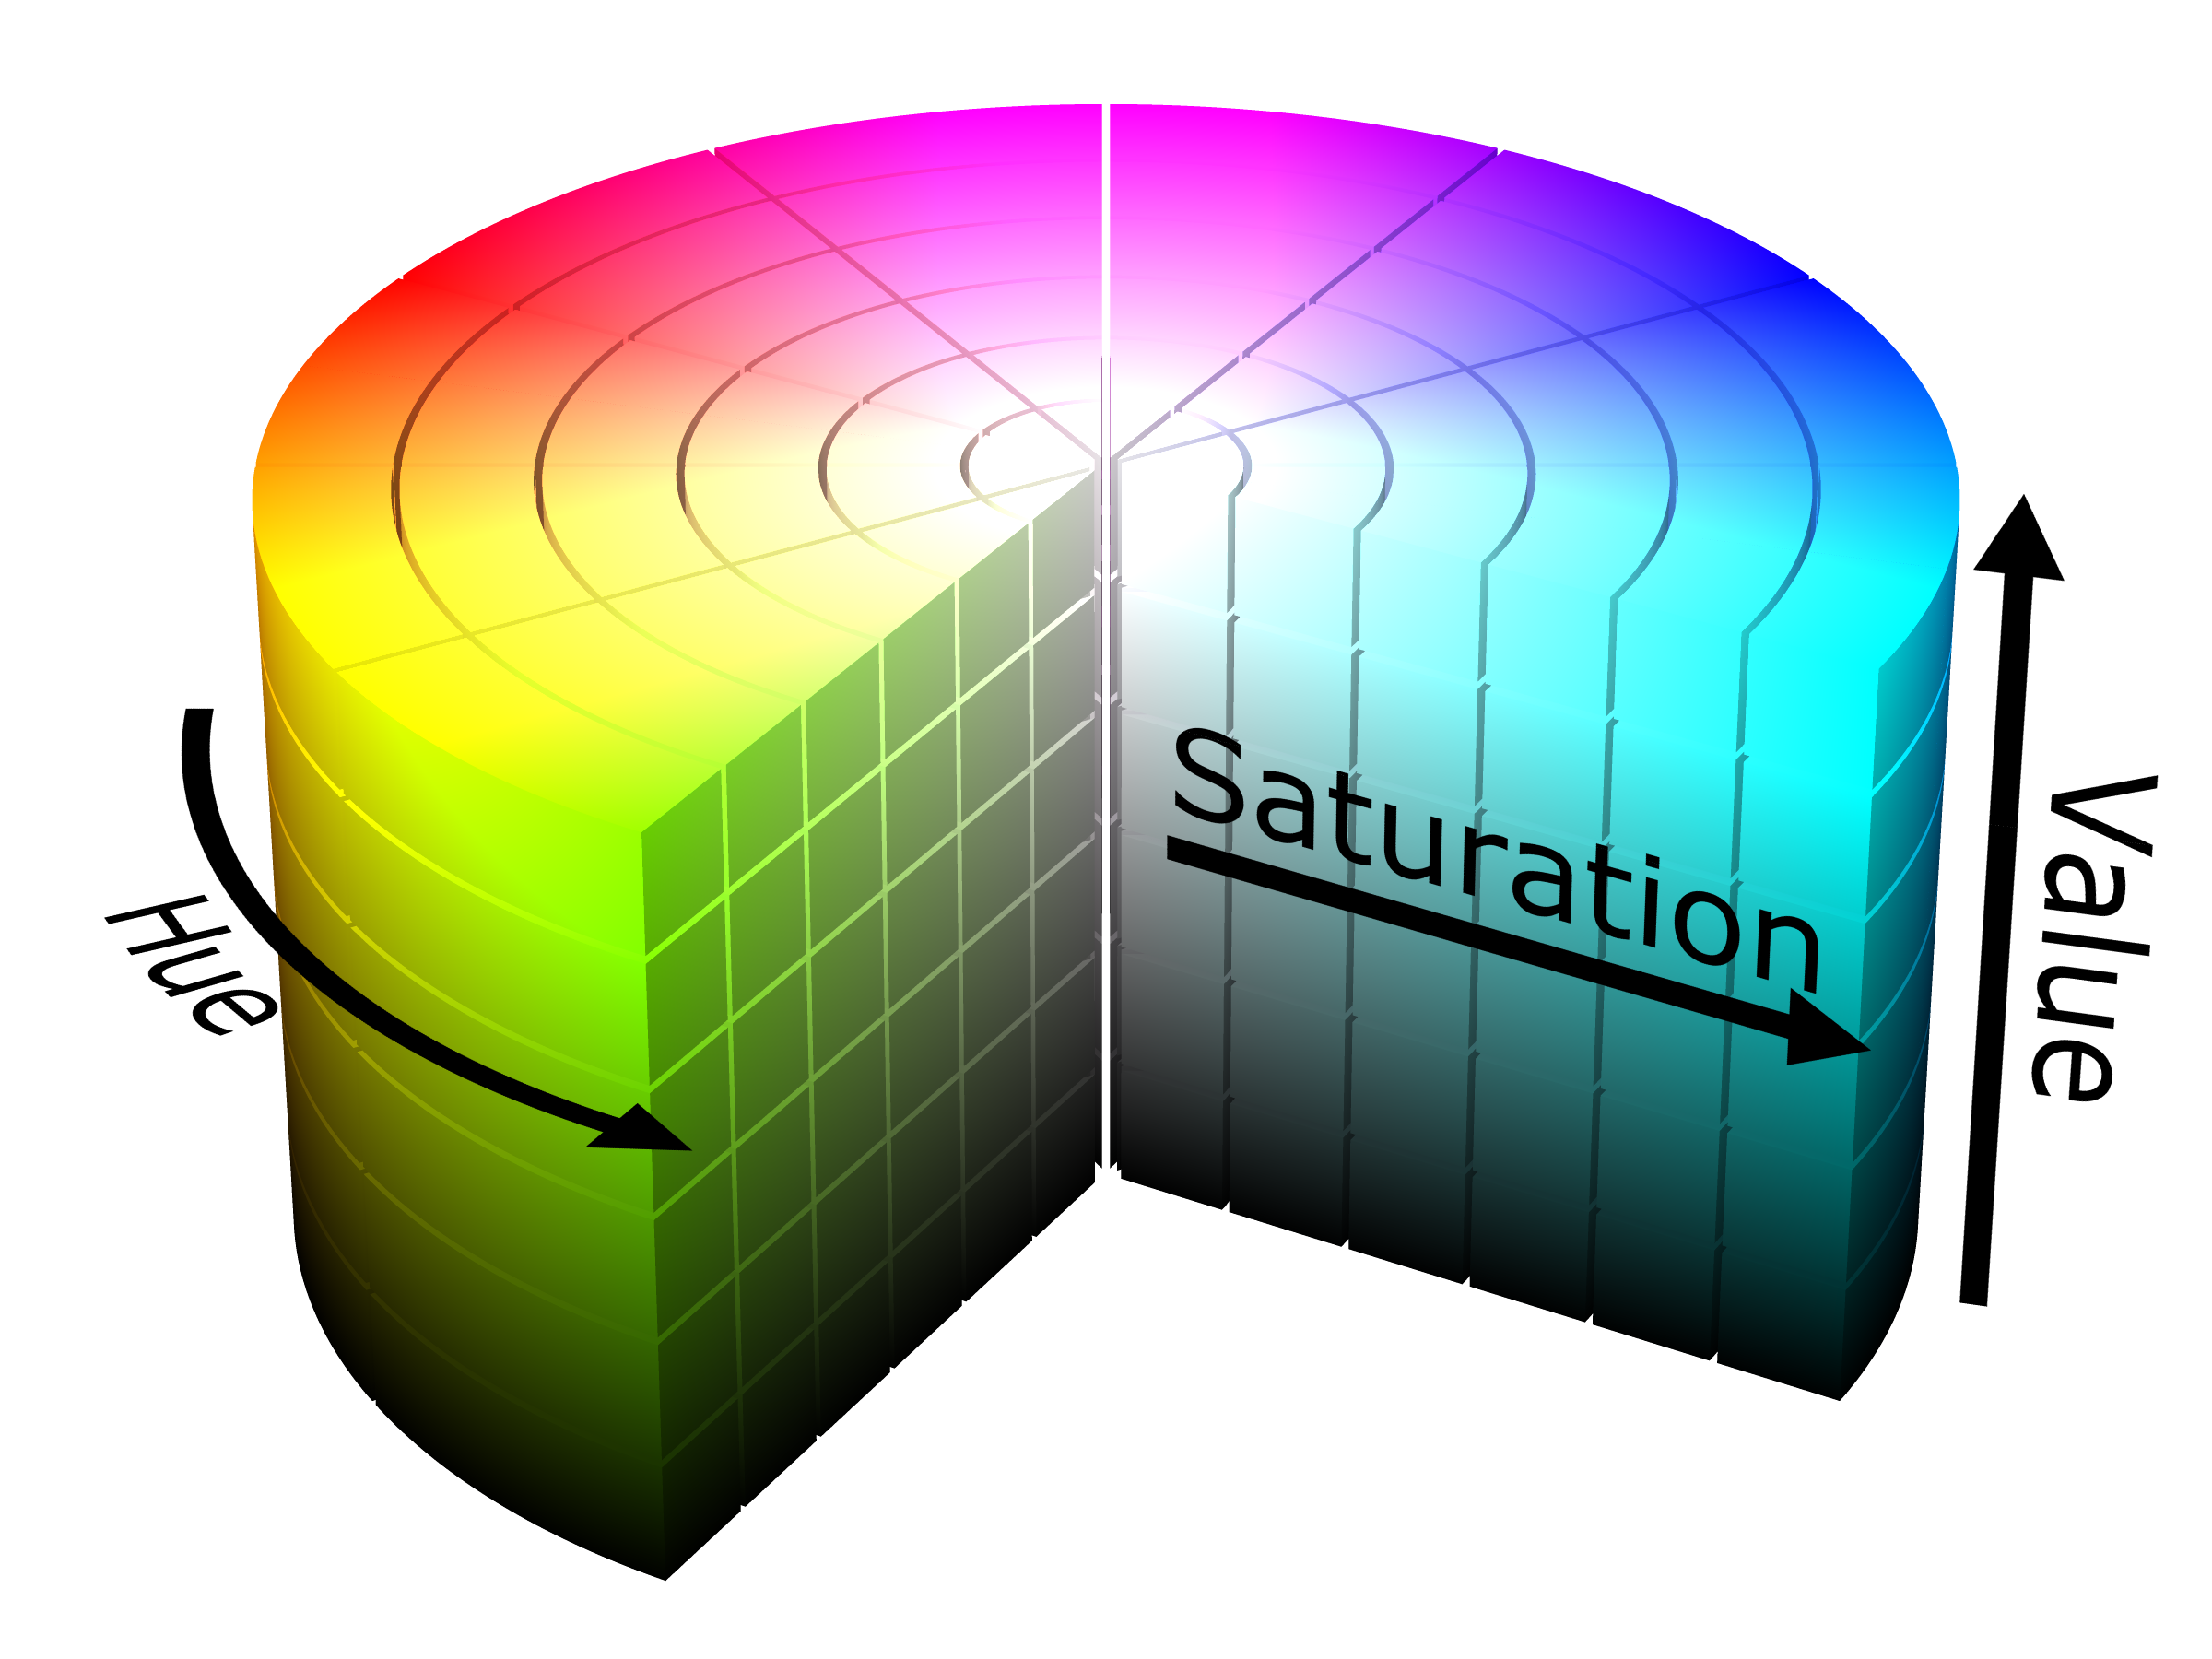
\includegraphics[scale=0.07]{HSV_Zylinder} 
\subsubsection{Anwendung im Code}
\lstinputlisting[language=Python, linerange={2-7}]{listings.py}
Zuerst wurden für jedes Feld auf dem Würfel die RGB-Werte von 400 Pixeln ausgelesen, danach die Durchschnitte davon genommen und in einer Liste gespeichert. Anschliessend können die RGB-Werte noch in den HSV-Farbraum umgerechnet werden. 
\lstinputlisting[language=Python, linerange={10-19}]{listings.py}
Um eine Seite nun einer Mitte zuzuordnen, werden die Abstände der eigenen Farbwerte zu den Farbwerten einer Mitte berechnet und die Quadrate davon addiert. Dies wird mit allen Mitten gemacht und schlussendlich wird die Seite derjenigen Mitte zugeordnet, bei der diese addierten Abstände am kleinsten waren.
\subsubsection{Vergleich}
Jetzt, wo die Farbräume und Methodik der Zuordnung klar sind, stellt sich die Frage, was die besten Ergebnisse liefert. Hierfür wurden fünf Ideen ausprobiert:
\begin{enumerate}
  \item Die RGB-Werte verwenden
  \item Die HSV-Werte verwenden
  \item Nur Hue und Saturation verwenden
  \item Nur Hue und Value verwenden
  \item Nur Hue verwenden
\end{enumerate}
Diese fünf Methoden wurden alle auf zehn Bilder von Rubiks Cubes angewandt, und anschliessend wurde ermittelt, wie viele Fehler die Methoden im Schnitt hatten. 

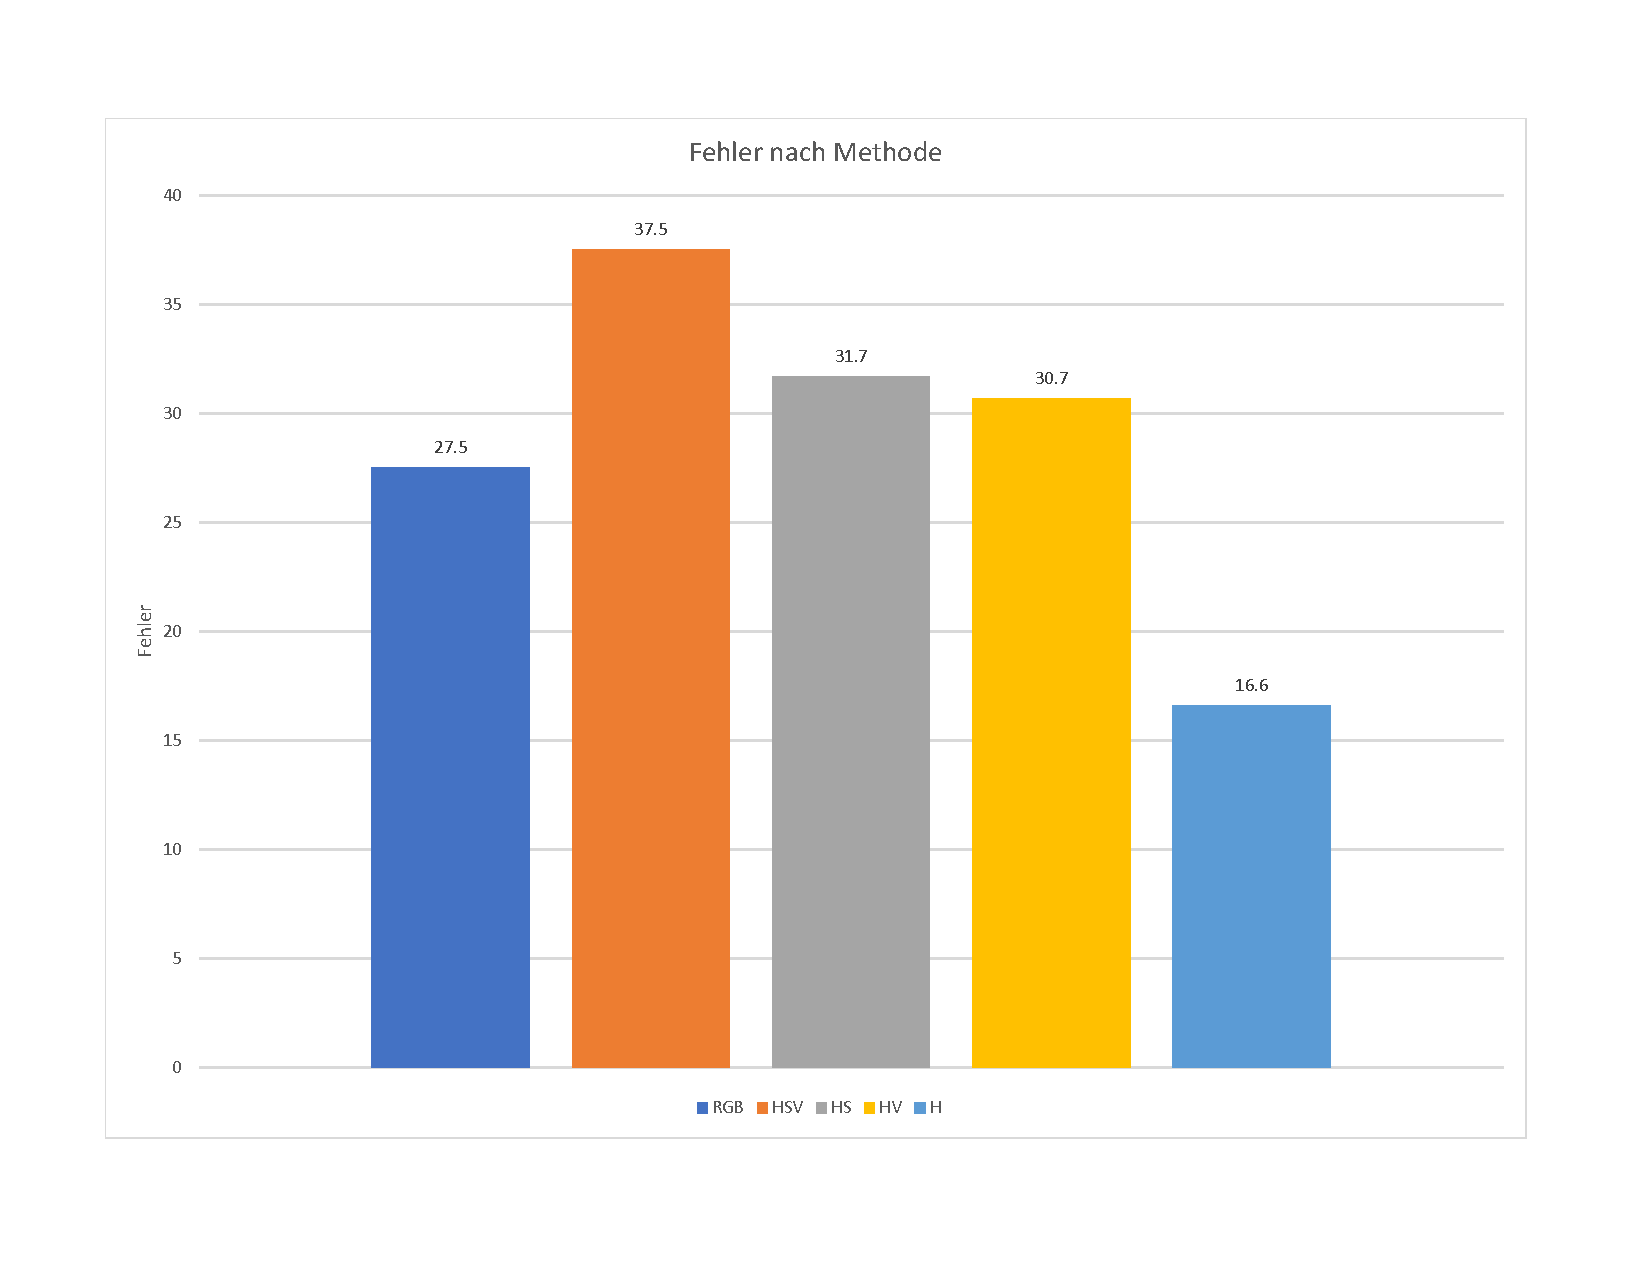
\includegraphics[scale=0.4]{Fehler_nach_Methode}

Wie im obigen Diagramm zu sehen, lieferte die Methode 5 die besten Ergebnisse, mit durchschnittlich 16.6 Fehlern bei 54 Feldern auf einem Würfel. Am zweitbesten war die RGB-Methode, mit jedoch fast doppelt so vielen Fehlern. Danach kamen nahe beieinander die Methoden 3 und 4, und schliesslich mit am meisten Fehlern die Methode 2. Dass die Methoden, die Saturation und/oder Value verwendeten, schlechter abschnitten, wie wenn nur Hue verwendet wurde war zu erwarten. Die Farben auf dem Würfel sind abgesehen von Weiss alle sehr satt und brillant. Wenn nun auf dem Bild eine Seite leicht überbelichtet oder schattig ist, dann verändert sich die Saturation oder der Value des Pixels. Somit werden dann zwei eigentlich identisch-farbige Felder als unterschiedlich angesehen, nur weil die Beleuchtung nicht identisch war. Diese Unterschiede werden bei Methode 5 nicht berücksichtigt, da nur die Hue-Werte verglichen werden. Auch die RGB-Methode erhält auf diese Weise Fehler. Da diese keine dedizierten Variablen für Sättigung und Helligkeit haben, verändern sich alle drei Variablen, wenn ein Feld andere Belichtung hat. Da sich diese Veränderung aber auf drei Variablen aufteilt, sind die einzelnen Werte nicht so weit entfernt, wie die von Saturation und Value. Und da die Quadrate der Entfernungen addiert werden, wirken sich zwei sehr falsche Werte mehr aus, als drei leicht falsche Werte. 

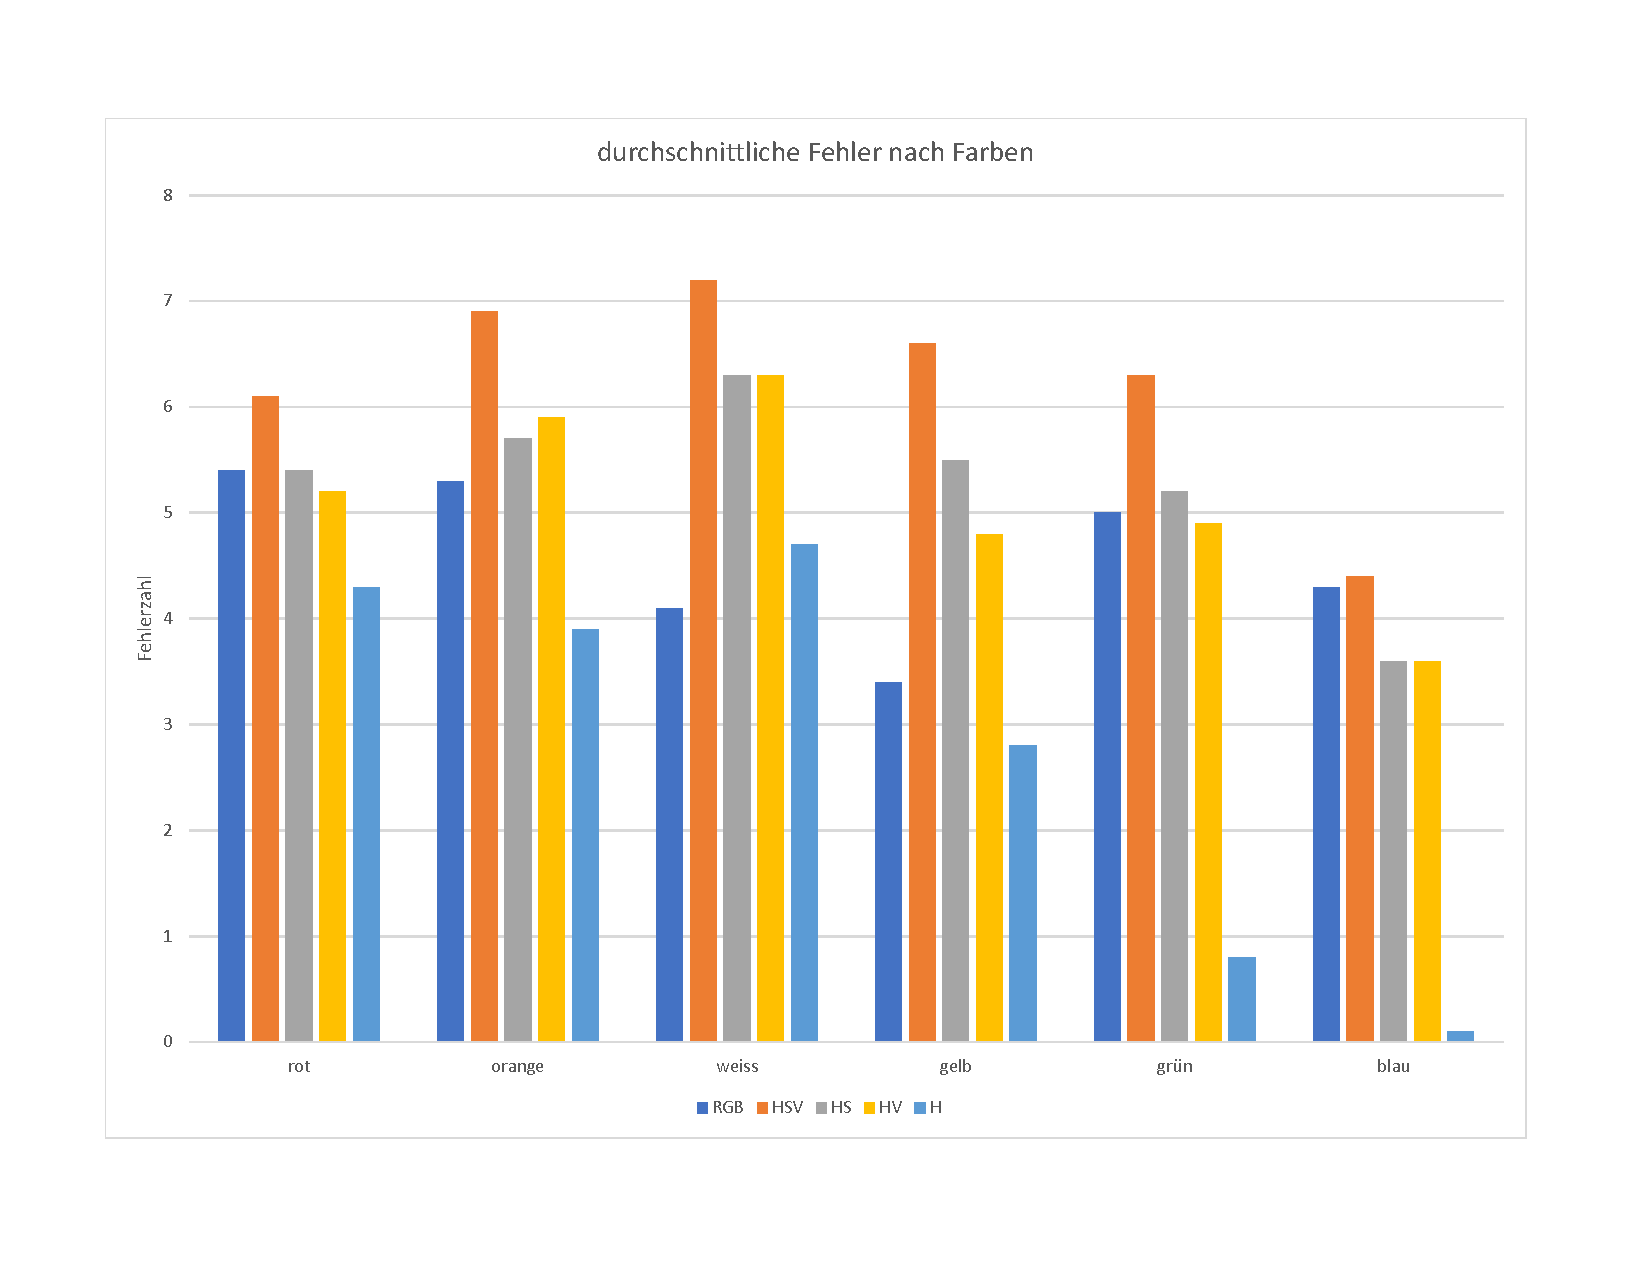
\includegraphics[scale=0.4]{durchschnittliche_Fehler_nach_Farben}

Wenn man die Fehler nun nach Farben aufteilt, sieht man, dass die Methode 5 bei allen Farben die beste ist, ausser bei Weiss, wo RGB besser funktioniert. Dies lässt sich dadurch erklären, dass Weiss im HSV-Farbraum dann entsteht, wenn die Saturation 0 ist. Wenn etwas also komplett weiss ist, dann bedeutet dies, dass der Hue-Wert nicht definierbar ist. Das Programm erkennt somit einen zufälligen Farbton, wenn es ein weisses Feld erkennen muss. Das Programm hat somit keine richtige Möglichkeit, die weissen Felder nur anhand des Farbtons zuzuordnen, weshalb es dort zu überdurchschnittlich vielen Fehlern kommt. 
\subsection{Saturation/Value weg}
\subsubsection{Problem}
Wie im letzten Abschnitt erwähnt, ergibt sich, wenn nur Hue zur Unterscheidung der Farben verwendet wird, das Problem, dass wenn die Saturation einer Farbe sehr tief ist, die Hue-Werte fast nicht erkannt werden können. Das gleiche gilt auch für zu tiefe Value-Werte. Diese Felder müssen also auf eine andere Weise bestimmt werden. 
\subsubsection{Lösung}
Dieses Problem kann behoben werden, indem die weissen und die (falls vorhandenen) schwarzen Felder schon aussortiert werden, bevor die restlichen Felder einer Mitte zugeordnet werden.
\lstinputlisting[language=Python, linerange={23-26}]{listings.py}
Zuerst werden alle Felder durchgegangen und es wird geschaut, ob sie einen festgelegten tiefen Saturation- oder Value-Wert unterschreiten. Danach wird geschaut, wie viele Felder einen tiefen Value besitzen. Falls es exakt neun sind, dann werden diese als schwarz eingestuft und beim anschliessenden zuordnen der Felder zu einer Mitte nicht mehr berücksichtigt. Wenn kein Feld einen tiefen Value hat, passiert nichts spezielles, da keine schwarzen Felder vorhanden sind. Falls aber irgend eine andere Anzahl Felder einen tiefen Value besitzen, stoppt das Programm, da die Anzahl schwarzer Felder nicht aufgeht, und Felder mit einem tiefen Value nicht unterscheidbar sind und der Würfel somit nicht verlässlich erkannt werden kann.
\lstinputlisting[language=Python, linerange={30-39}]{listings.py}
 Nachdem die schwarzen Felder aussortiert worden sind, geschieht das gleiche mit den weissen Feldern, die eine tiefe Saturation haben. 
 
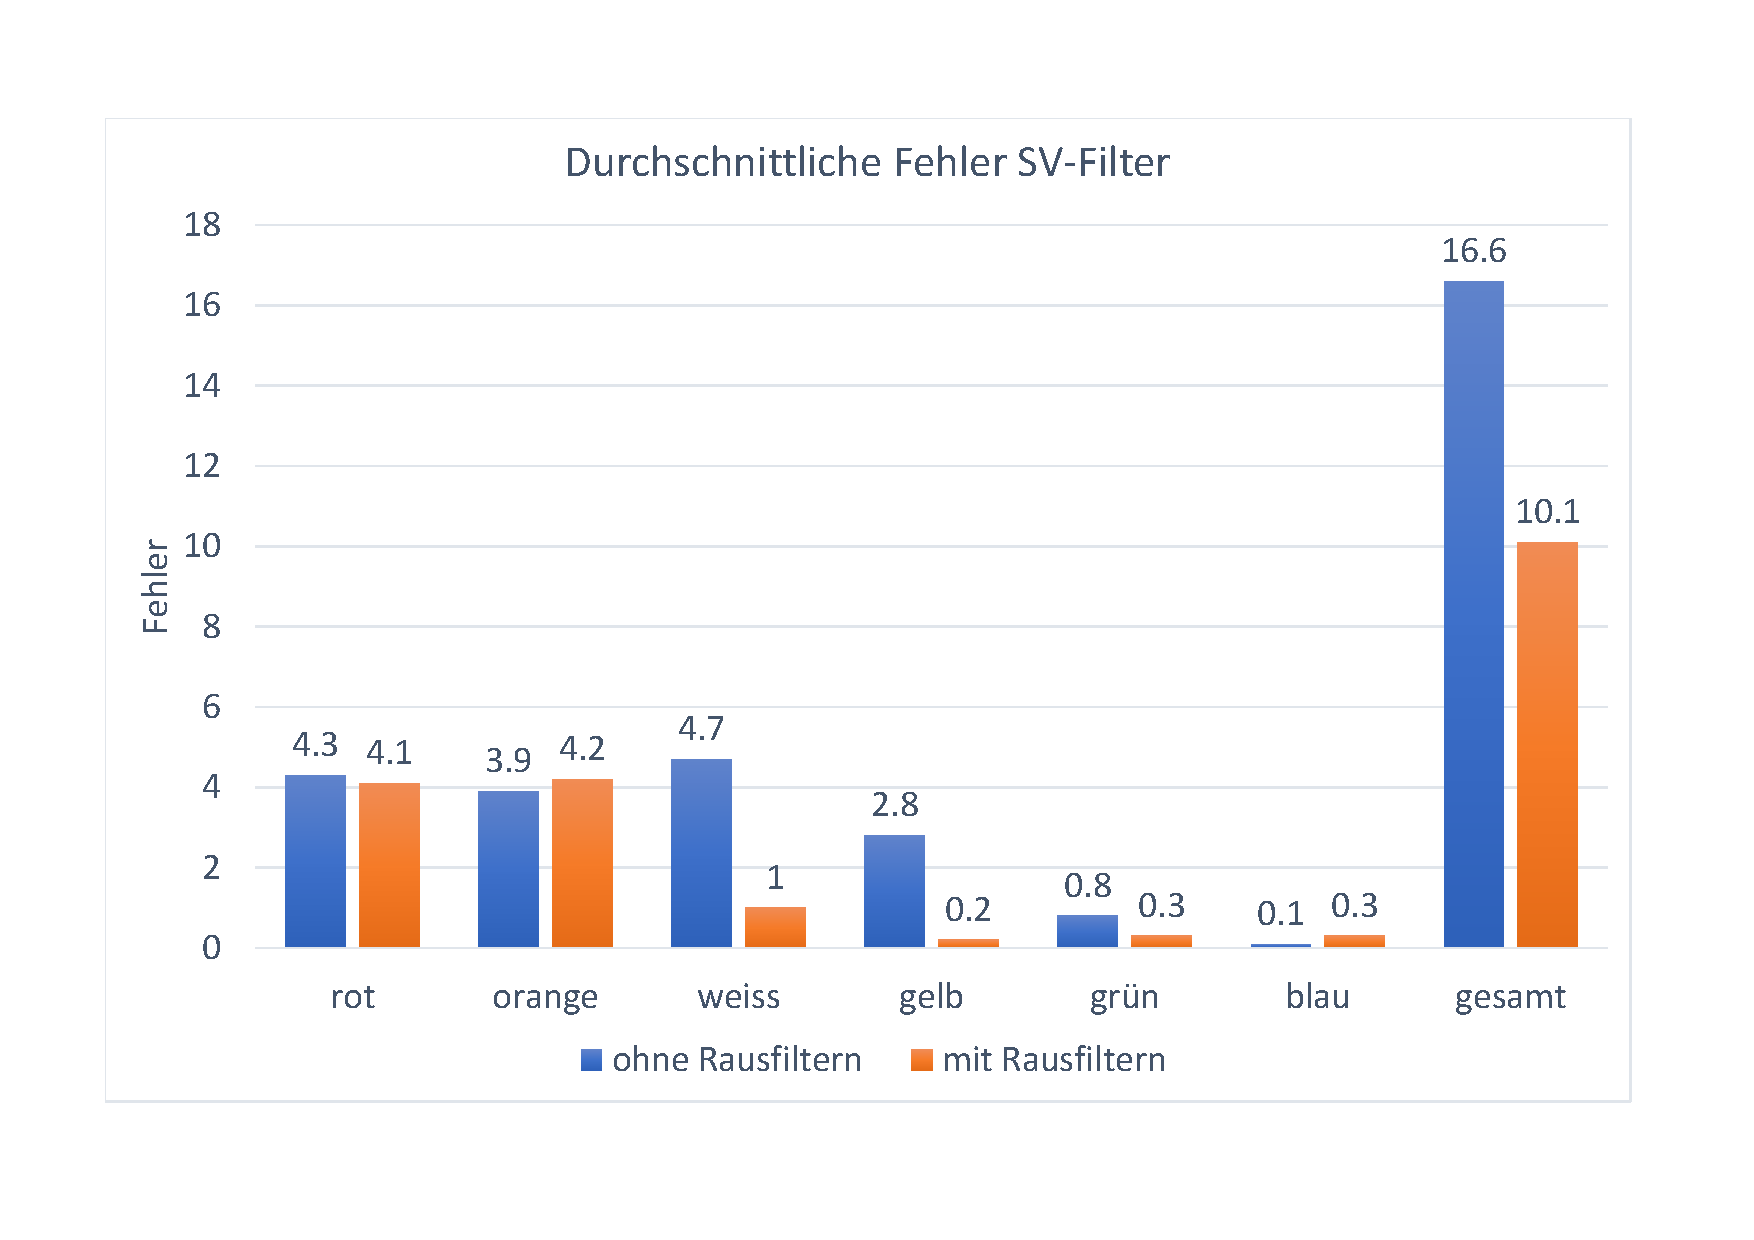
\includegraphics[scale=0.4]{Fehler_SV_Filter} 

Durch das Anwenden dieser Filter, sinkt die durchschnittliche Fehlerzahl von 16.6 auf 10.1 Fehler auf 54 Felder. Diese Verbesserung kommt hauptsächlich wegen den weissen und gelben Feldern zustande. Von den weissen Feldern wird neu nur noch eins statt 4.7 falsch erkannt, und bei den Gelben sind es statt 2.8 noch 0.2 Fehler.
\subsection{richtige Anzahl Felder pro Farbe}
Da bei einem Rubiks Cube bekannt ist, dass jede Farbe exakt neun mal vorkommt, weiss man, dass jeder Mitte exakt acht Felder zugeordnet werden müssen. Ist dies nach der Zuordnung nicht der Fall, lässt sich daraus schliessen, dass der Würfel noch nicht korrekt erkannt ist. In so einem Fall kann man nun noch einen Algorithmus einfügen, der dafür sorgt, dass jede Farbe exakt neun mal vorkommt. Dafür wurden zwei verschiedene Methoden ausprobiert.
\subsubsection{nah an Mitte}
Die erste Methode ist die, die in den bisherigen Vergleichen auch schon angewandt wurde. Sie funktioniert so, dass wenn einer Mitte zu viele Steine zugeordnet werden, wird geschaut welcher dieser Steine am nächsten bei einer Mitte ist, der noch zu wenige Steine zugeordnet worden sind. Dieser Vorgang wird so lange wiederholt, bis der Mitte nur noch acht Seitensteine zugeordnet sind. Dann geht das Programm weiter zur nächsten Mitte, der zu viele Steine zugeordnet sind, bis allen Mitten exakt acht Seitensteine zugeordnet sind. 
\lstinputlisting[language=Python, linerange={44-64}]{listings.py}
\subsubsection{weit weg von Mitte}
Die zweite Methode funktioniert folgendermassen. Es werden ebenfalls die Mitten durchgegangen, denen zu viele Flächen zugeordnet wurden. Aber statt iwe bei Methode eins zu schauen, welche Fläche am nächsten bei einer anderen Mitte ist, wird geschaut, welche Fläche am weitesten entfernt von der eigenen Mitte ist. Diese wird dann derjenigen Mitte zugeordnet, die noch zu wenig Flächen hat und der sie am nächsten ist.
\lstinputlisting[language=Python, linerange={69-89}]{listings.py}
\subsubsection{Vergleich}

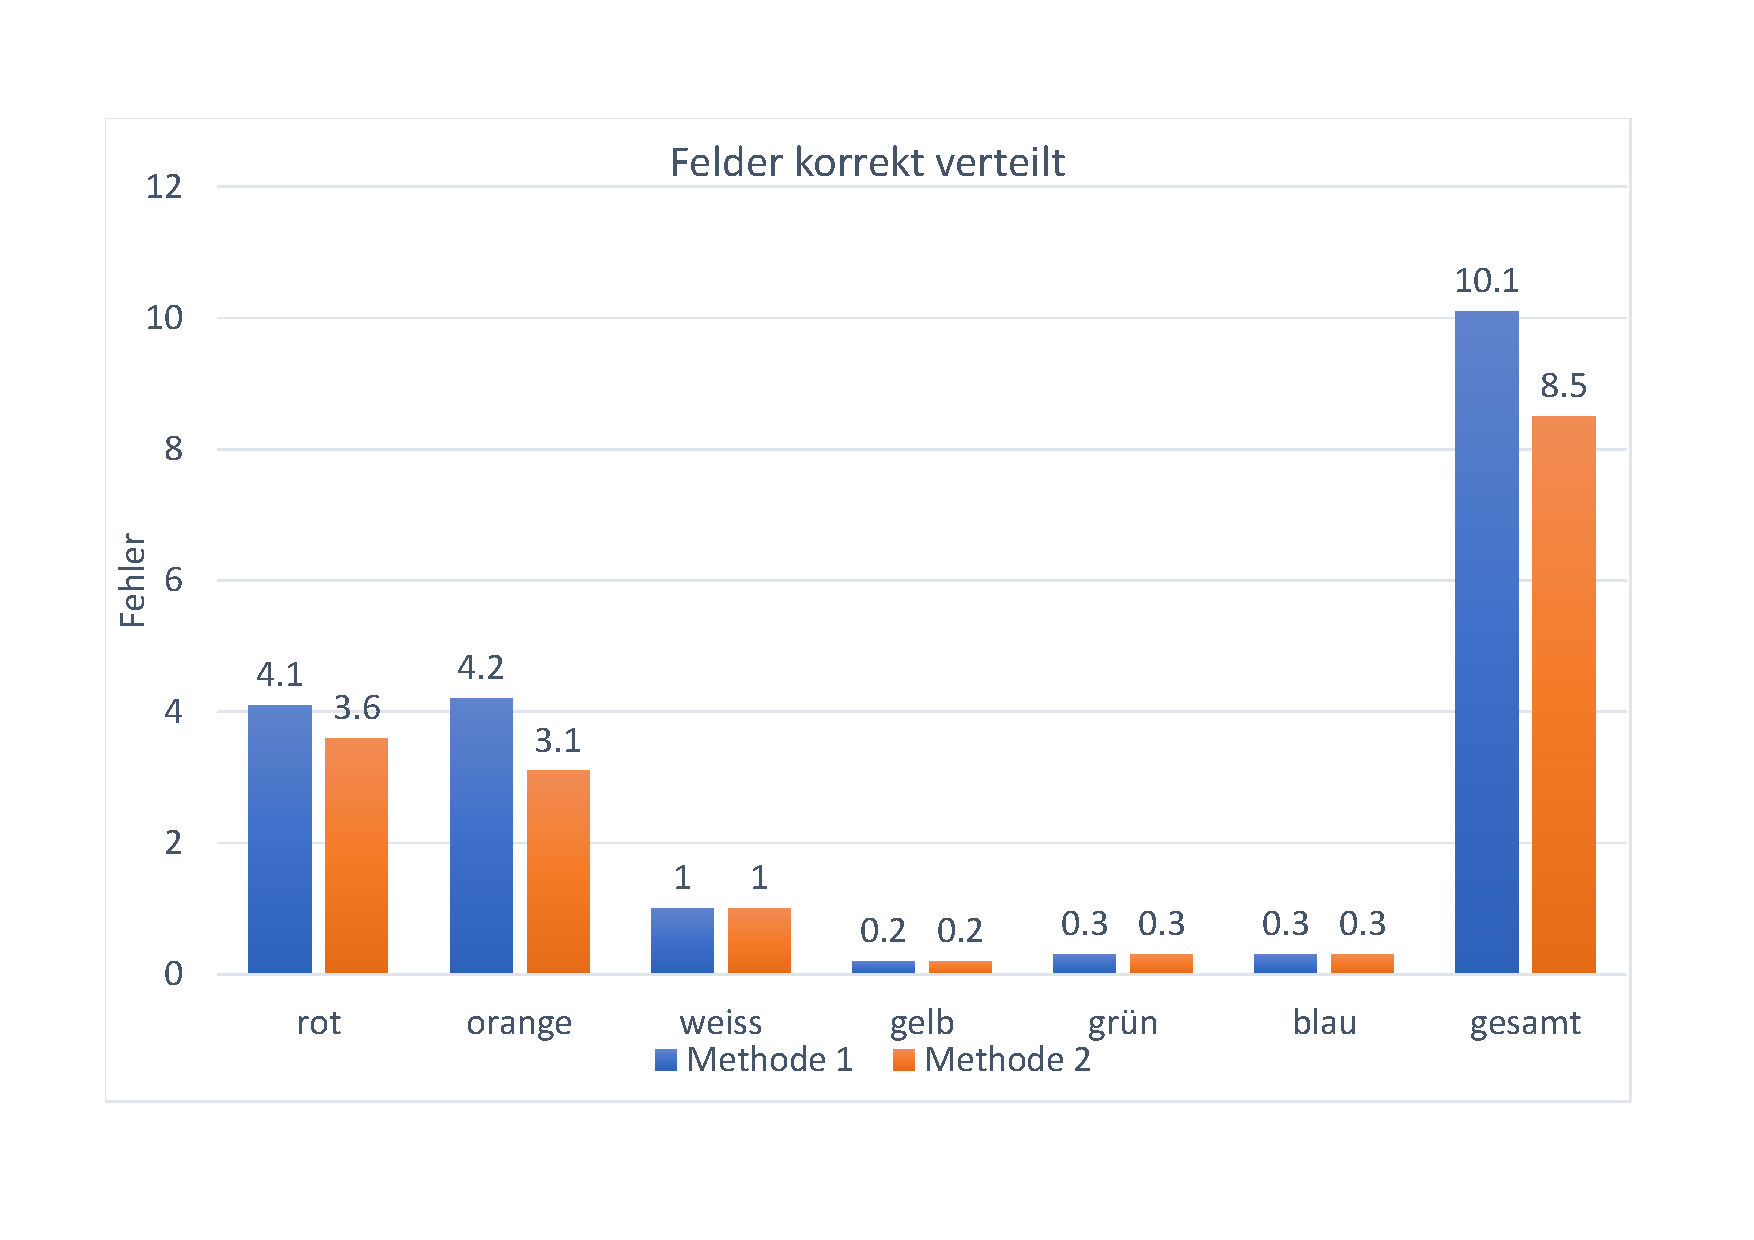
\includegraphics[scale=0.4]{Felder_korrekt_verteilt}

Wie im Diagramm zu sehen liefert die Methode 2 die besseren Resultate. Der Unterschied kommt jedoch nur bei den roten und orangen Feldern zustande. Bei allen anderen Farben sind die beiden Methoden gleich gut. 
\subsection{Wahrscheinlichkeit}
\subsubsection{Idee}
\subsubsection{logistische Funktion}
\section{Schluss}
Um hier noch einmal die Resultate zusammenzufassen: Es war immer ziemlich deutlich, welche Ideen besser waren, wie die anderen. Die besten Ergebnisse kamen heraus, wenn zuerst die weissen und schwarzen Felder herausgefiltert werden, danach die Felder anhand des Hue-Wertes zugeordnet werden, und dann schliesslich bei denen Farben, denen zu viele Felder zugeordnet wurden, die Felder, die am weitesten von der Mitte entfernt sind, noch umgeordenet werden. Aber auch dann gibt es im Schnitt noch 8.5 Fehler. Dies zeigt, dass es sehr schwierig ist, ein verlässliches Programm zu erstellen, welches den Rubiks Cube perfekt erkennt. Ein grosser Faktor, der dabei eine wichtige Rolle spielt, sind die Lichtverhältnisse. wenn die verschiedenen Seiten auch nur schon einen kleinen Unterschied in der Beleuchtung haben, kann es zu Fehlern kommen. Es wird versucht, diese zu minimieren, indem nur Hue als Unterscheidungsmerkmal verwendet wird, aber es entstehen trotzdem noch Fehler. Es gibt aber noch einige Ideen, die die Anzahl Fehler möglicherweise noch reduzieren könnten. Zum Beispiel könnte noch geschaut werden, ob das erkannte Muster überhaupt entstehen kann, wenn ein Rubiks Cube vermischt wird. Es ist beispielsweise nicht möglich, dass auf einem Eckstein eine Farbe mehrmals vorkommt. Es kann auch noch weiter erforscht werden, wie die Veränderung der Lichtverhältnisse die erkannten Farben verändert. Es wäre auch möglich einen komplett anderen Ansatz zu versuchen, indem man ein neuronales Netz verwendet. Hier käme einfach das Problem hinzu, dass das Trainieren eines neuronalen Netzes, möglicherweise hunderte oder tausende von Bildern benötigt, was sehr aufwendig wäre. 
\end{document}
